\chapter{Methodes Agiles}\label{agile}
L'équipe dans laquelle je fais mon stage utilisent les méthodes Agiles(cf. lexique \ref{lexique:agile} p.\pageref{lexique:agile}) et eXtreme Programming(cf. lexique \ref{lexique:XP} p.\pageref{lexique:XP}) en particulier. Ces méthodes ne sont pas figées et doivent être adaptées à chaque équipe. Il est donc courant et primordial que certaines pratiques soient remises en cause (cf. tableau \ref{tableau:evolPratXP} p.\pageref{tableau:evolPratXP}. Ce chapitre donne un aperçu des pratiques XP utilisées par l'équipe R\&D de SMARTESTING dans le cadre du développement de la solution Smartesting.

% Le projet est stocké sur un serveur Subversion\footnote{}
%TRAC, SVN, HUDSON, Jira, IntelliJ Idea, Ubuntu 8.10, RSM 7.0.0.x, 7.0.5, 7.5, Together 2007,2008, RQM, HP Mercury Quality Center, HP Quick Test Center.
%Travail sur IDEA, svn
%TODO : mise en place, utilisation, utilité ...

\section{Itération}
L'équipe organise son travail sous forme d'itérations d'une semaine. Chaque itération traite un nombre de fonctionnalités limité qui est quantifié en points de vélocité(cf. lexique \ref{lexique:velocité} p.\pageref{lexique:velocité}). À la fin de mon stage la vélocité variait entre 7 et 13 points par semaine. Une itération est planifiée lors de la rétrospective de l'itération précédente. Un itération compte un certain nombre de points de vélocité qui constitue une estimation de la durée requise pour développer les fonctionalités planifiées. La durée d'une itération à la première semaine de mon stage etait de deux semaines. Elle est tout de suite passée à une semaine. À la fin d'une itération le produit est livré. Les versions mineures sont disponibles pour les consultants afin de les tester sur le terrain et d'obtenir des retours en condition réele. Les versions majeures de fin de jalon (Milestone) bénéficient d'une période de validation approfondie et sont disponibles aux utilisateurs finaux.

\begin{figure}[!h]
\centering
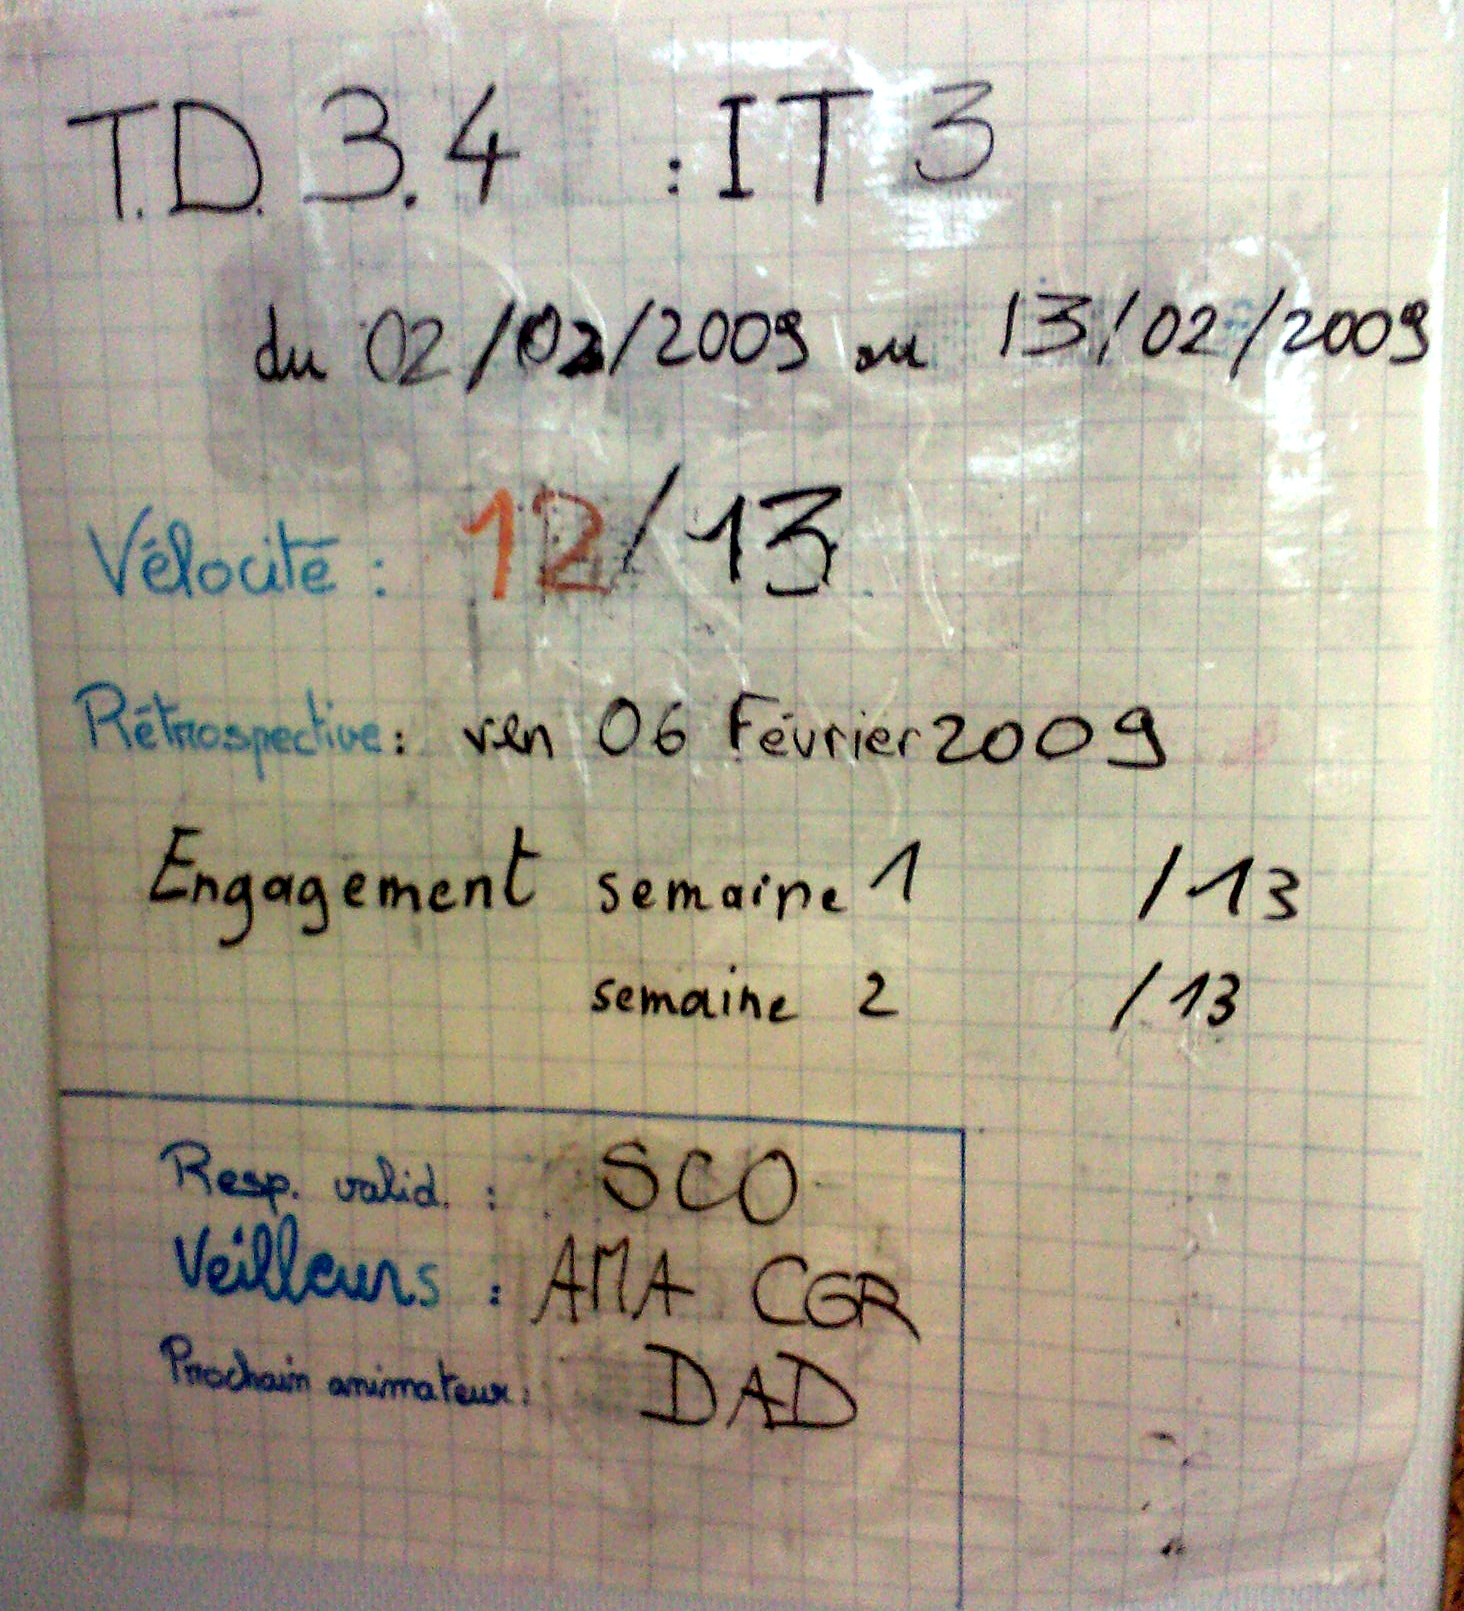
\includegraphics[scale=0.10]{Illustrations/SP_A0182.jpg}
\caption{Iteration}
\label{fig:Iteration}
\end{figure}

\section{Rétrospective}
Lors de la rétrospective d'une itération, les membres de l'équipe de R\& D se réunissent pour parler de la précédente itération et pour planifier celle à venir. La réunion commence par un ``check in'' pendant lequel une question est posée (par exemple ``Comment voyez vous Test Designer dans un an?'') en général afin de se remémorer l'itération (se remettre mentalement dedans). Un point est sur des statistiques (métriques) telles que le nombre de lignes de code,la couverture de tests unitaires(cf. lexique \ref{lexique:testU} p.\pageref{lexique:testU}) et haut niveau(cf. lexique \ref{lexique:testHL} p.\pageref{lexique:testHL}) ou encore la vélocité atteinte par rapport aux objectifs. L'attention est ensuite portée sur les fonctionnalités qui ont été réalisées ou non lors de l'itération. La réunion se continue par les discussions diverses, chacun peut discuter de diverses choses : apparition de problèmes, amélioration du fonctionnement de l'équipe. La réunion se termine enfin par l'annonce de la prochaine vélocité et l'attribution des responsabilités pour l'itération qui vient. En effet chaque itération a des responsables différents (animateur de la rétrospective, validation, veilleur ...)

\section{Fiches}\label{agile:fiches}
Des fiches correspondent aux différentes tâches à effectuer dans le cadre d'une itération. Elles peuvent être de type différent : valeur client (couleur blanche), Tâche technique (couleur verte), Point technique (couleur bleue), Anomalie (couleur rouge), Amélioration de process / Prototype (couleur jaune). Les couleurs des fiches permettent à l'équipe d'identifier au premier coup d'oeil le travail à réaliser et l'urgence. Si le tableau comporte beaucoup de fiches rouges, elles seront à traiter en priorité car ce sont des anomalies. Les fiches possèdent des points de vélocité qui correspondent à la quantité de travail à effectuer (en demie-journée par binôme) sur la tâche. Si la fiche est trop importante elle peut être redécoupées en fiches plus petites.

\begin{figure}[!h]
\centering
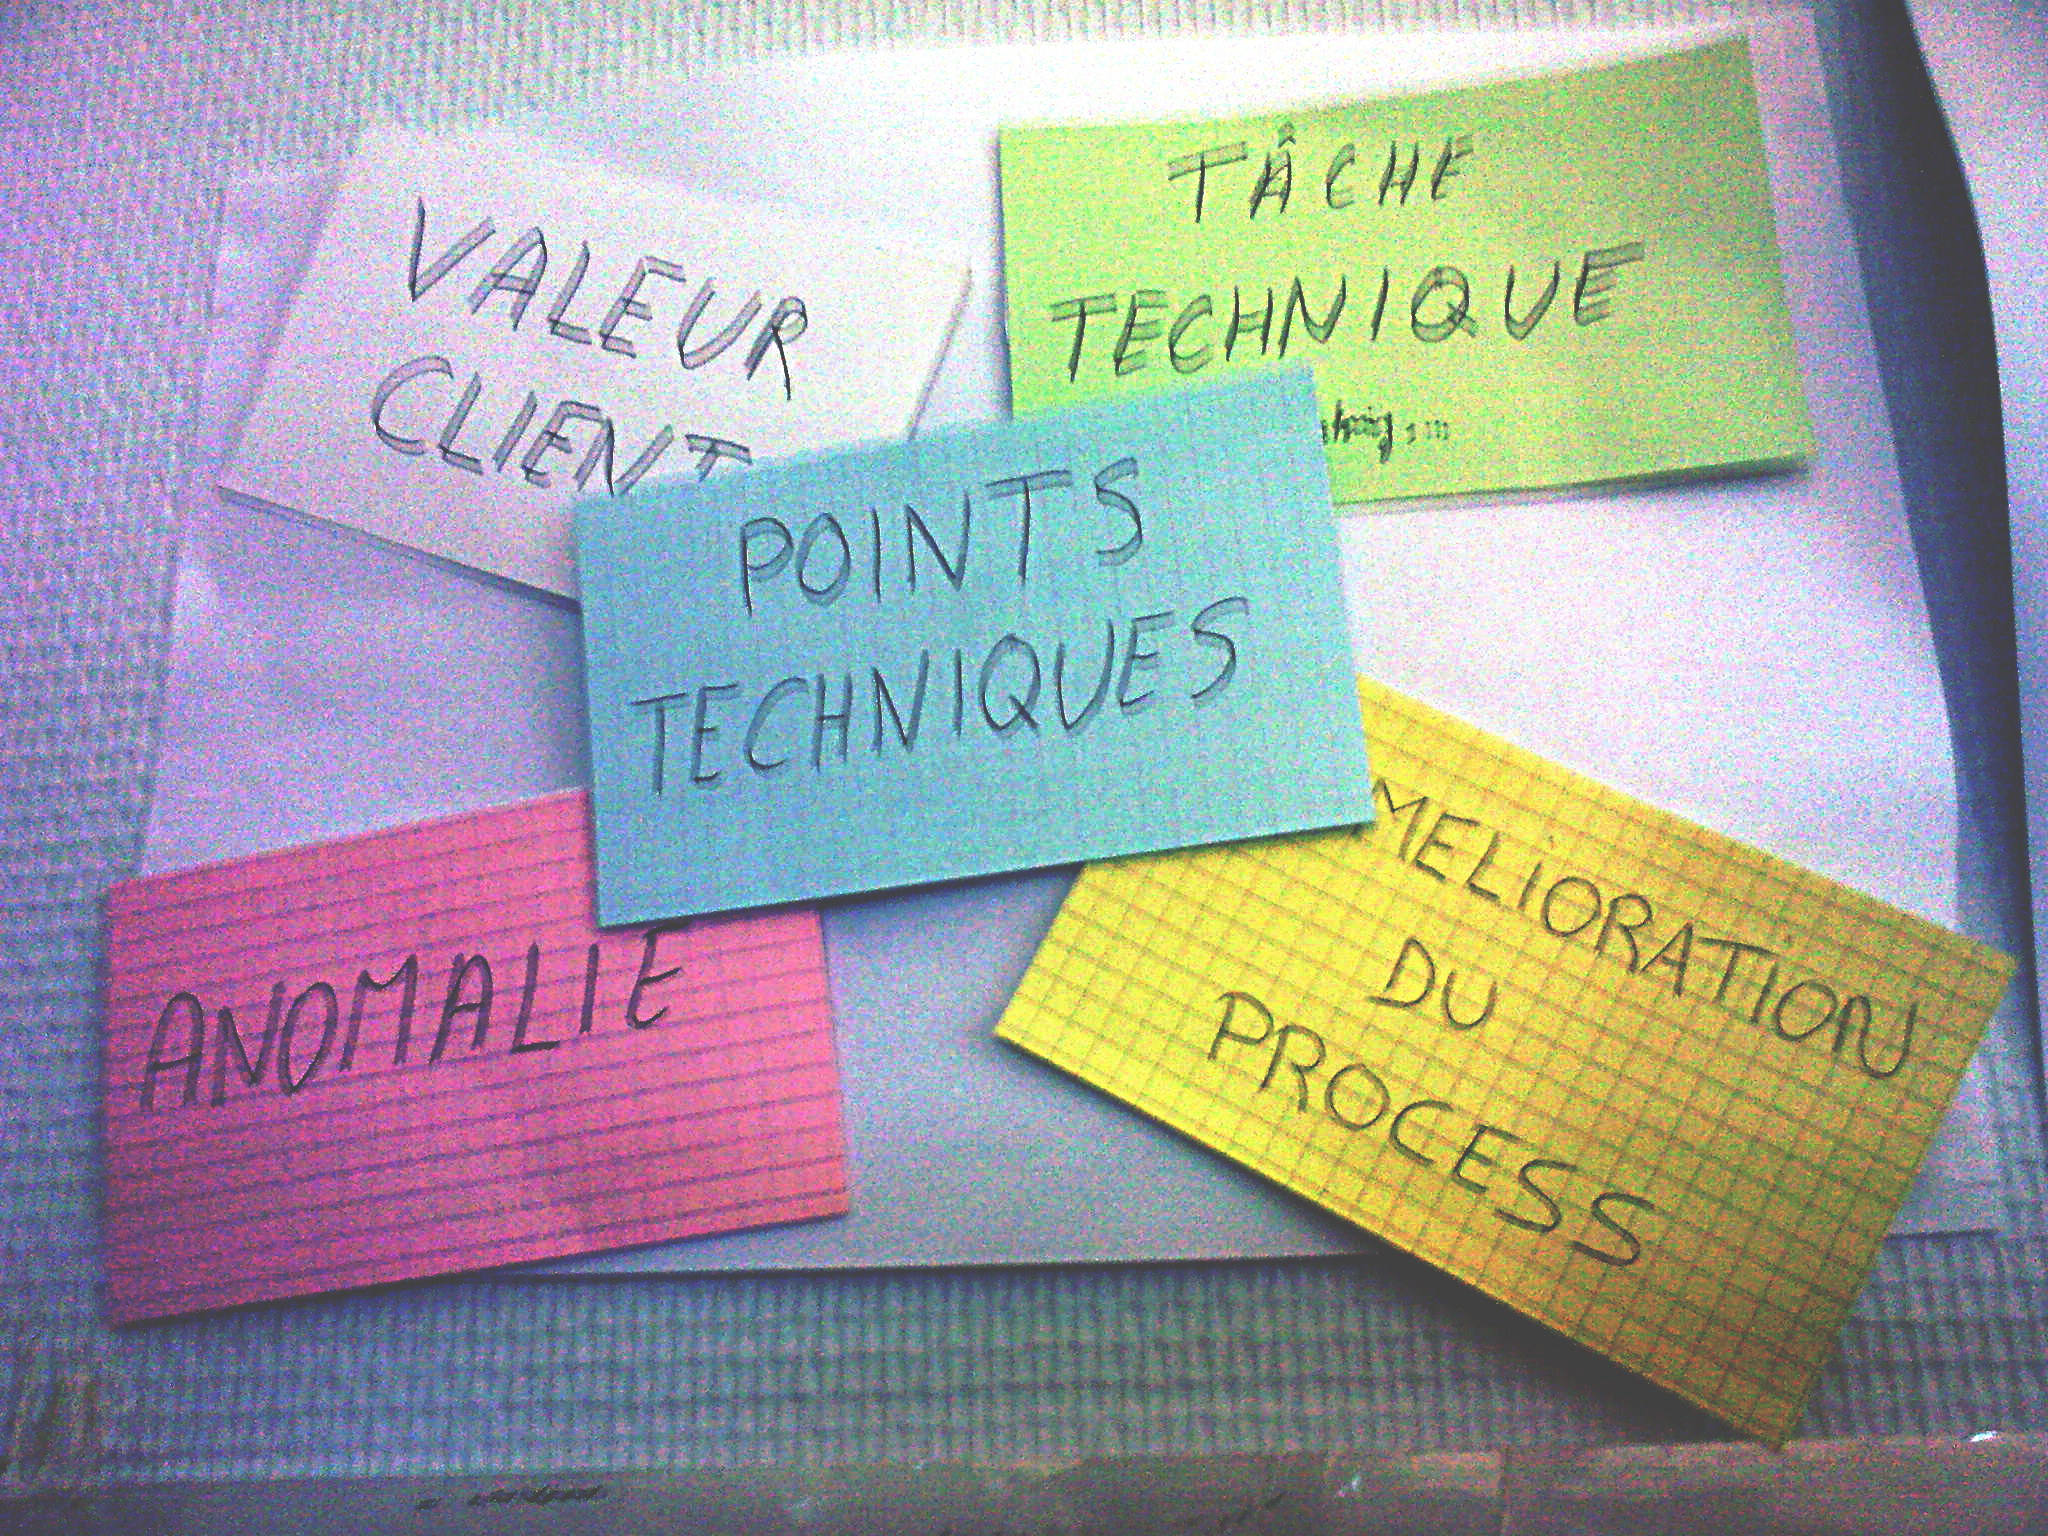
\includegraphics[scale=0.10]{Illustrations/SP_A0185.jpg}
\caption{Fiches}
\label{fig:Fiches}
\end{figure}

\begin{figure}[!h]
\centering
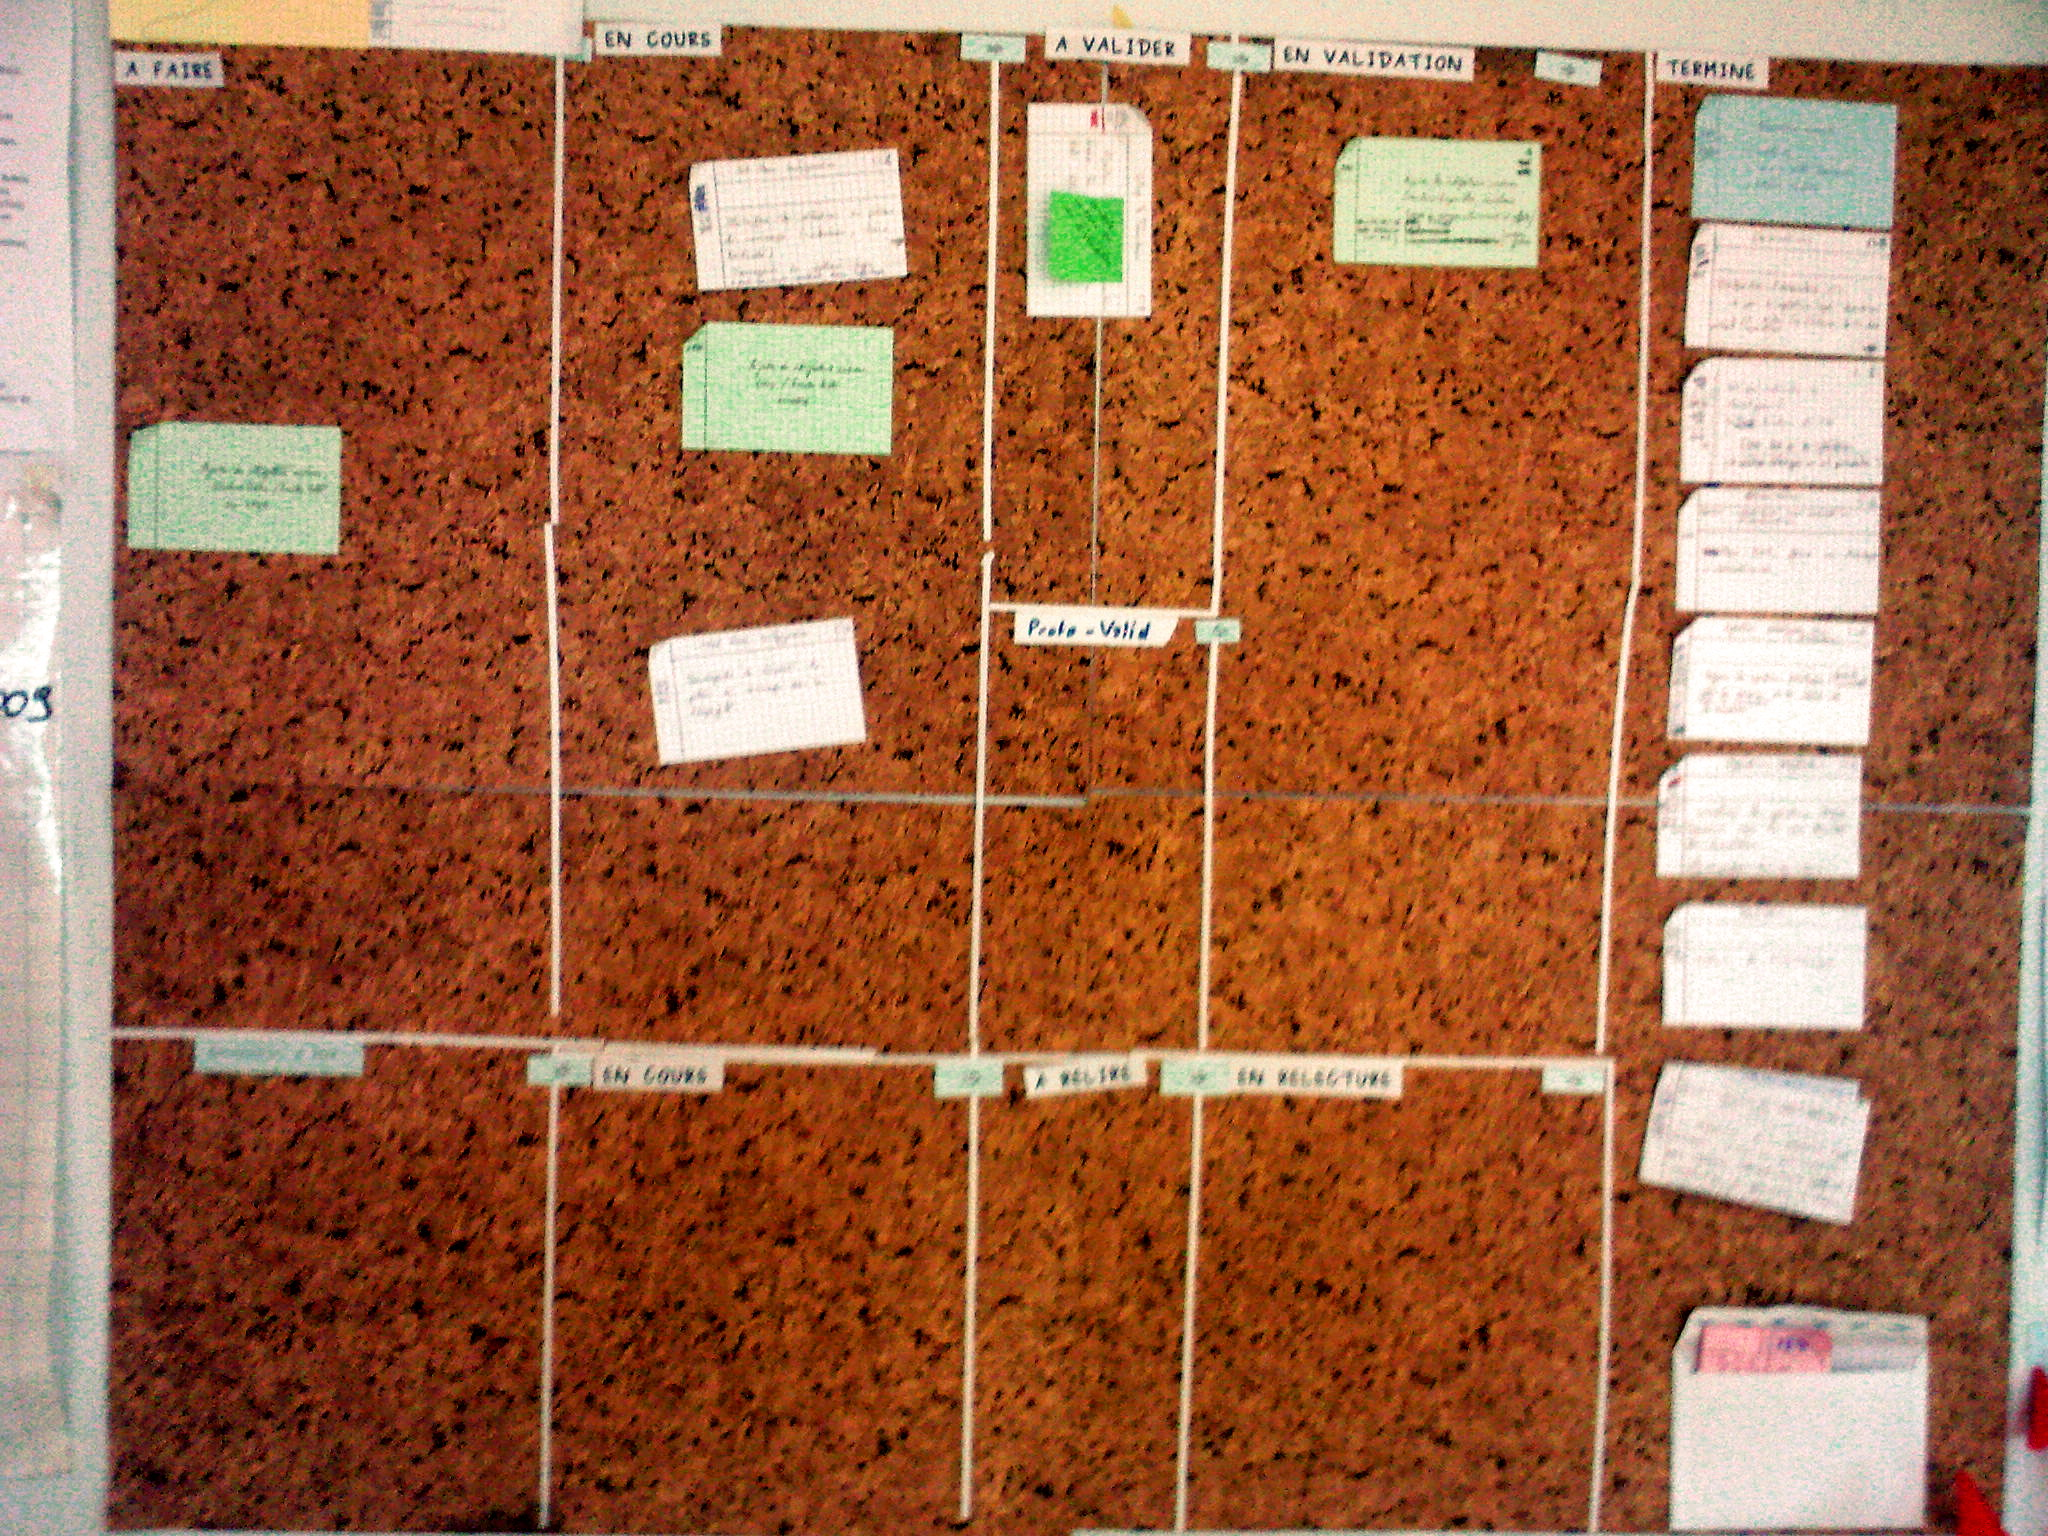
\includegraphics[scale=0.10]{Illustrations/SP_A0183.jpg}
\caption{Tableau d'avancement des fiches}
\label{fig:Tableau d'avancement des fiches}
\end{figure}

\section{Travail en binômes (pair programming)}
Une grand partie du travail dans l'équipe est réalisée en binôme. Les binômes changent très souvent. Les avantages du travail en binôme sont multiples. Contrairement à la programmation individuelle les binômes permettent de diffuser plus rapidement le savoir acquis lors du développement et seront plus à même à partager leur connaissances (effet boule de neige). De plus des études montrent que le travail par paires donne généralement un code de meilleure qualité, une meilleure capture des bugs. La communication et la motivation dans l'équipe sont également améliorées par cette méthode. Chaque personne dans le binôme peut prendre le clavier et la souris pour donner ses idées de développement. En général le travail en binôme est un échange d'idées permanent. Chaque binôme, en début de fiche s'engage sur cette fiche et estime le temps qui lui sera necessaire pour la terminer. Cette estimation est revue régulièrement (lors du morning meeting par exemple) et est communiquée à l'équipe et au client XP.

\begin{figure}[!h]
\centering
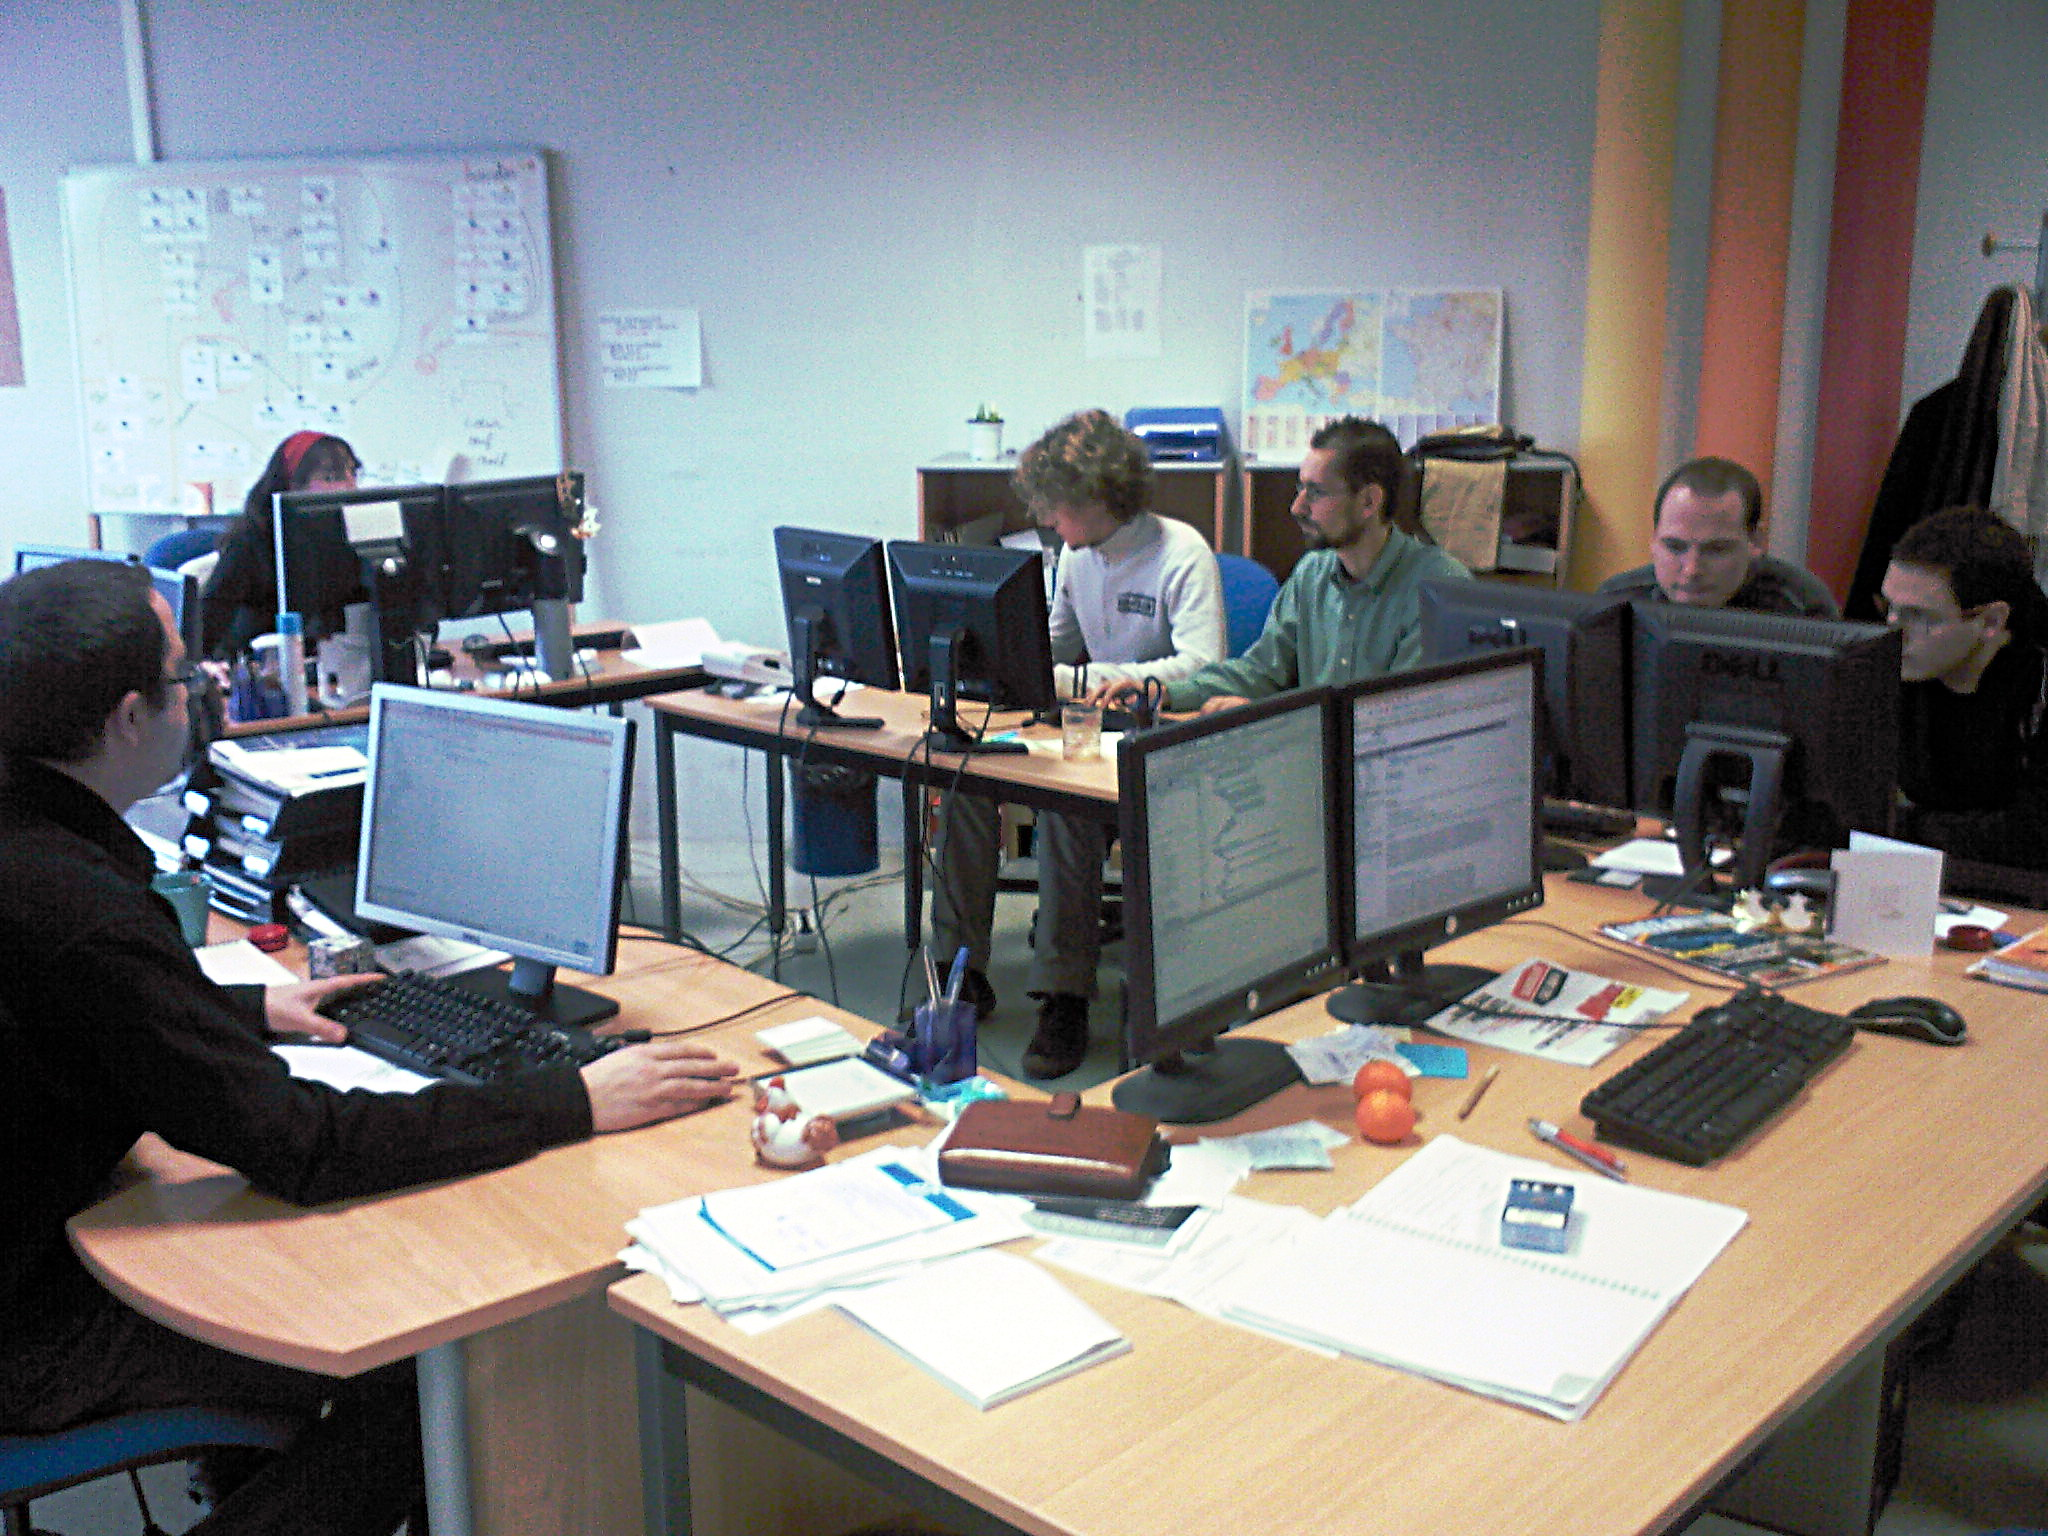
\includegraphics[scale=0.15]{Illustrations/SP_A0188.jpg}
\caption{Pair programming}
\label{fig:Pair programming}
\end{figure}

\section{Validation}
La validation joue un rôle important lors de l'itération. Une partie de la validation est réalisée en permanence par les serveurs d'intégration continue. Une autre partie (en général, l'utilisation via l'interface homme-machine) ne peut être réalisée que par des personnes qui n'ont pas participé au développement de la fonctionnalité. Cela permet d'avoir une idée plus objective des manipulations à effectuer pour tester la fonctionnalité. Au cours de la semaine la validation est la tâche exclusive de Batman. Il valide une fiche dès qu'elle a été mise ``À valider'' afin d'avoir le retour le plus rapide sur la fonctionnalité. Lors de la validation, on fait très souvent appel au client XP pour vérifier que la fonctionnalité correspond bien aux besoin énoncés. À la fin de l'itération, lorsque toute les fiche sont terminées et validées, l'équipe commence une validation de l'ensemble des fiches de l'itération. Lorsque toute l'équipe est satisfaite (les bugs éventuels corrigés, documentation relue ...) la livraison peut avoir lieu.

\section{Semaine type}
La semaine Agile à la R\&d de SMARTESTING est rythmée par quelques pratiques qui peuvent évoluer.
\subsection*{Cotation et engagement}
Avant de commencer une itération, l'egagement est fait. C'est à dire que les fiches qui vont déterminer les développements de la semaine vont être choisies par le client XP. Les fiches sont posées sur le tableau en vue de tous. La somme des vélocités des fiches correspond à la vélocité déterminée lors de la retrospective de l'itération précédente. L'équipe peut alors choisir les fiches qui seront commencées dans la semaine, les binômes se créent. Chaque binôme va ensuite voir le client XP afin de confirmer le périmètre fonctionnel de la fiche. 

\subsection{Morning meeting}
Les membres de l'équipe se réunissent juste avant la pause déjeuner pour parler de ce qu'ils ont fait la matinée. Toute l'équipe est réunie en cercle et se fait passer un objet. Celui qui a l'objet prend la parole. Chaque binôme informe toute l'équipe de l'avancée de son engagement ainsi que des problèmes qu'il rencontre. Le temps de parole est très bref et si un problème mérite une attention particulière il sera traité hors du cercle plus tard. Après le tour du cercle s'il y a des informations complémentaires à mentionner elles le sont. Le meeting se termine ensuite par une pensée du jour.

\subsubsection{Point perso}
Le mardi, juste avant la pause déjeuner, un membre de l'équipe fait une présentation à l'aide d'un projecteur sur un sujet de son choix (pas nécessairement lié à l'informatique d'ailleurs). La présentation doit durer 10 minutes. À la fin, les membres de l'équipe peuvent poser des questions et commenter la manière dont la présentation a été réalisée (Intéresser le public, parler clairement, qualité du support...). Cet exercice de communication permet aux membres de l'équipe d'apprendre à partager et à structurer leurs idées. Cela peut être très utile lors de manifestations diverses (xp days, agile tour...). Le point perso a évolué entre le début et la fin de mon stage, et actuellement différentes nouvelles formes en sont expérimentées.

\subsubsection{Discussion sur un livre}
L'équipe lit un livre pendant la semaine et se réunit le mercredi avant la pause de midi pour commenter un chapitre. L'équipe lorsque je suis arrivé lisait ``The Art of Agile Development''. Cette activité permet deja de lire en anglais , mais également d'améliorer la cohésion de l'équipe par l'éventuelle adoption de pratiques nouvelles. Plusieurs des pratiques évoquées dans ce livre ont été adoptées après mon arrivée. Ce fut le cas de ``No bugs'', ``Done-done'', ``Slack time'' par exemple. Cette pratique a disparu avec le temps car plusieurs personnes de l'équipe n'y trouvaient plus d'intérêt.

\subsection{Point technique}
Le Jeudi matin en début de matinée a lieu le point technique il peut varier dans son contenu. Cela peut aller de la discussion d'un point technique rencontré lors de l'itération à un code contest de 30 minutes.

